\documentclass[tikz,border=2mm]{standalone}
\usetikzlibrary{arrows,calc}
\usepackage{anyfontsize}
\newcommand{\jiuhao}{\fontsize{2.55pt}{\baselineskip}\selectfont}
\newcommand{\shihao}{\fontsize{1.2pt}{\baselineskip}\selectfont}
\begin{document}
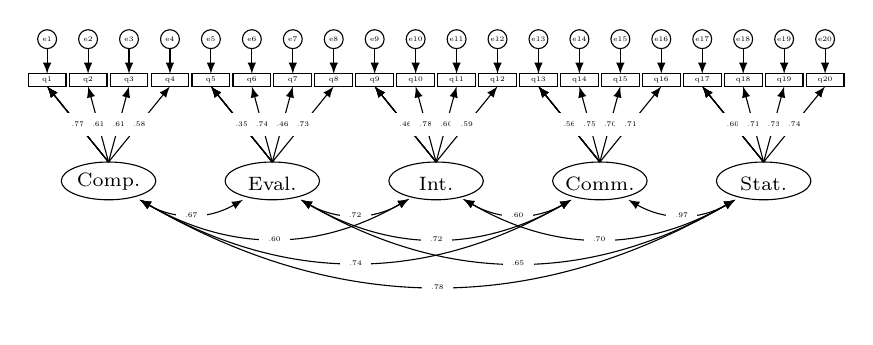
\begin{tikzpicture}[scale=0.4]
%draw circles with adjusted spacing to align with rectangles
\foreach \i in {1,...,20}
\draw (1.3*\i,10.5) circle [radius=0.3] node[font=\jiuhao] {e{\i}};
%draw rectangles with increased width and spacing
\foreach \i in {1,...,20}
    \draw (1.3*\i-0.6,9) rectangle (1.3*\i+0.6,9.4) ;
\foreach \i in {1,...,20}
    \node at (1.3*\i,9.2)[font=\jiuhao]{q{\i}};
%draw ellipses
\draw (3.25,6) ellipse (1.5 and 0.6);
\draw (8.45,6) ellipse (1.5 and 0.6);
\draw (13.65,6) ellipse (1.5 and 0.6);
\draw (18.85,6) ellipse (1.5 and 0.6);
\draw (24.05,6) ellipse (1.5 and 0.6);
% draw arrows
\foreach \i in {1,...,20}
\draw [-latex] (1.3*\i,10.2) -- (1.3*\i,9.4);
\foreach \i in {1,...,4}
%\draw [-latex] (3,6.6) -- (\i,9);
\draw [-latex] (3.25,6.6) to node[fill=white,font=\jiuhao]{.77} (1.3,9);
\draw [-latex] (3.25,6.6) to node[fill=white,font=\jiuhao]{.61} (2.6,9) ;
\draw [-latex] (3.25,6.6) to node[fill=white,font=\jiuhao]{.61} (3.9,9) ;
\draw [-latex] (3.25,6.6) to node[fill=white,font=\jiuhao]{.58} (5.2,9) ;
\foreach \i in {5,...,8}
% Arrows from the second ellipse to the center of rectangles 5 to 8
\draw [-latex] (8.45,6.6) to node[fill=white, font=\jiuhao]{.35} (6.5,9);
\draw [-latex] (8.45,6.6) to node[fill=white, font=\jiuhao]{.74} (7.8,9);
\draw [-latex] (8.45,6.6) to node[fill=white, font=\jiuhao]{.46} (9.1,9);
\draw [-latex] (8.45,6.6) to node[fill=white, font=\jiuhao]{.73} (10.4,9);
\foreach \i in {9,...,12}
% Arrows from the third ellipse to the center of rectangles 9 to 12
\draw [-latex] (13.65,6.6) to node[fill=white, font=\jiuhao]{.46} (11.7,9);
\draw [-latex] (13.65,6.6) to node[fill=white, font=\jiuhao]{.78} (13.0,9);
\draw [-latex] (13.65,6.6) to node[fill=white, font=\jiuhao]{.60} (14.3,9);
\draw [-latex] (13.65,6.6) to node[fill=white, font=\jiuhao]{.59} (15.6,9);
\foreach \i in {13,...,16}
% Arrows from the fourth ellipse to the center of rectangles 13 to 16
\draw [-latex] (18.85,6.6) to node[fill=white, font=\jiuhao]{.56} (16.9,9);
\draw [-latex] (18.85,6.6) to node[fill=white, font=\jiuhao]{.75} (18.2,9);
\draw [-latex] (18.85,6.6) to node[fill=white, font=\jiuhao]{.70} (19.5,9);
\draw [-latex] (18.85,6.6) to node[fill=white, font=\jiuhao]{.71} (20.8,9);
\foreach \i in {17,...,20}
% Arrows from the fifth ellipse to the center of rectangles 17 to 20
\draw [-latex] (24.05,6.6) to node[fill=white, font=\jiuhao]{.60} (22.1,9);
\draw [-latex] (24.05,6.6) to node[fill=white, font=\jiuhao]{.71} (23.4,9);
\draw [-latex] (24.05,6.6) to node[fill=white, font=\jiuhao]{.73} (24.7,9);
\draw [-latex] (24.05,6.6) to node[fill=white, font=\jiuhao]{.74} (26.0,9);
\node[above] (a) at (3.25,5.4) [font=\scriptsize] {Comp.};
\node[above] (b) at (8.45,5.4) [font=\scriptsize] {Eval.};
\node [above](c) at (13.65,5.4) [font=\scriptsize]{Int.};
\node [above](d) at (18.85,5.4) [font=\scriptsize]{Comm.};
\node[above] (e) at (24.05,5.4) [font=\scriptsize]{Stat.};
%\draw[<->,-latex] (a) -- (b);
\draw[<->,>=latex,bend right]  (a) to node[fill=white,font=\jiuhao] {.67} (b) ;
\draw[<->,>=latex,bend right]  (b) to node[fill=white,font=\jiuhao] {.72} (c);
\draw[<->,>=latex,bend right]  (c) to node[fill=white,font=\jiuhao] {.60} (d);
\draw[<->,>=latex,bend right]  (d) to node[fill=white,font=\jiuhao] {.97} (e);
\draw[<->,>=latex,bend right]  (a) to node[fill=white,font=\jiuhao] {.60} (c);
\draw[<->,>=latex,bend right]  (a) to node[fill=white,font=\jiuhao] {.74} (d);
\draw[<->,>=latex,bend right]  (a) to node[fill=white,font=\jiuhao] {.78} (e);
\draw[<->,>=latex,bend right]  (b) to node[fill=white,font=\jiuhao] {.72} (d);
\draw[<->,>=latex,bend right]  (b) to node[fill=white,font=\jiuhao] {.65} (e);
\draw[<->,>=latex,bend right]  (c) to node[fill=white,font=\jiuhao] {.70} (e);

\end{tikzpicture}
%test sample
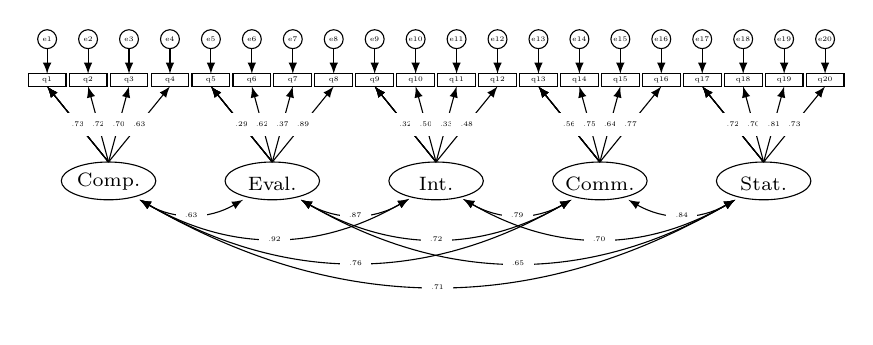
\begin{tikzpicture}[scale=0.4]
%draw circles with adjusted spacing to align with rectangles
\foreach \i in {1,...,20}
\draw (1.3*\i,10.5) circle [radius=0.3] node[font=\jiuhao] {e{\i}};
%draw rectangles with increased width and spacing
\foreach \i in {1,...,20}
    \draw (1.3*\i-0.6,9) rectangle (1.3*\i+0.6,9.4) ;
\foreach \i in {1,...,20}
    \node at (1.3*\i,9.2)[font=\jiuhao]{q{\i}};
%draw ellipses
\draw (3.25,6) ellipse (1.5 and 0.6);
\draw (8.45,6) ellipse (1.5 and 0.6);
\draw (13.65,6) ellipse (1.5 and 0.6);
\draw (18.85,6) ellipse (1.5 and 0.6);
\draw (24.05,6) ellipse (1.5 and 0.6);
% draw arrows
\foreach \i in {1,...,20}
\draw [-latex] (1.3*\i,10.2) -- (1.3*\i,9.4);
\foreach \i in {1,...,4}
%\draw [-latex] (3,6.6) -- (\i,9);
\draw [-latex] (3.25,6.6) to node[fill=white,font=\jiuhao]{.73} (1.3,9);
\draw [-latex] (3.25,6.6) to node[fill=white,font=\jiuhao]{.72} (2.6,9) ;
\draw [-latex] (3.25,6.6) to node[fill=white,font=\jiuhao]{.70} (3.9,9) ;
\draw [-latex] (3.25,6.6) to node[fill=white,font=\jiuhao]{.63} (5.2,9) ;
\foreach \i in {5,...,8}
% Arrows from the second ellipse to the center of rectangles 5 to 8
\draw [-latex] (8.45,6.6) to node[fill=white, font=\jiuhao]{.29} (6.5,9);
\draw [-latex] (8.45,6.6) to node[fill=white, font=\jiuhao]{.62} (7.8,9);
\draw [-latex] (8.45,6.6) to node[fill=white, font=\jiuhao]{.37} (9.1,9);
\draw [-latex] (8.45,6.6) to node[fill=white, font=\jiuhao]{.89} (10.4,9);
\foreach \i in {9,...,12}
% Arrows from the third ellipse to the center of rectangles 9 to 12
\draw [-latex] (13.65,6.6) to node[fill=white, font=\jiuhao]{.32} (11.7,9);
\draw [-latex] (13.65,6.6) to node[fill=white, font=\jiuhao]{.50} (13.0,9);
\draw [-latex] (13.65,6.6) to node[fill=white, font=\jiuhao]{.33} (14.3,9);
\draw [-latex] (13.65,6.6) to node[fill=white, font=\jiuhao]{.48} (15.6,9);
\foreach \i in {13,...,16}
% Arrows from the fourth ellipse to the center of rectangles 13 to 16
\draw [-latex] (18.85,6.6) to node[fill=white, font=\jiuhao]{.56} (16.9,9);
\draw [-latex] (18.85,6.6) to node[fill=white, font=\jiuhao]{.75} (18.2,9);
\draw [-latex] (18.85,6.6) to node[fill=white, font=\jiuhao]{.64} (19.5,9);
\draw [-latex] (18.85,6.6) to node[fill=white, font=\jiuhao]{.77} (20.8,9);
\foreach \i in {17,...,20}
% Arrows from the fifth ellipse to the center of rectangles 17 to 20
\draw [-latex] (24.05,6.6) to node[fill=white, font=\jiuhao]{.72} (22.1,9);
\draw [-latex] (24.05,6.6) to node[fill=white, font=\jiuhao]{.70} (23.4,9);
\draw [-latex] (24.05,6.6) to node[fill=white, font=\jiuhao]{.81} (24.7,9);
\draw [-latex] (24.05,6.6) to node[fill=white, font=\jiuhao]{.73} (26.0,9);
\node[above] (a) at (3.25,5.4) [font=\scriptsize] {Comp.};
\node[above] (b) at (8.45,5.4) [font=\scriptsize] {Eval.};
\node [above](c) at (13.65,5.4) [font=\scriptsize]{Int.};
\node [above](d) at (18.85,5.4) [font=\scriptsize]{Comm.};
\node[above] (e) at (24.05,5.4) [font=\scriptsize]{Stat.};
%\draw[<->,-latex] (a) -- (b);
\draw[<->,>=latex,bend right]  (a) to node[fill=white,font=\jiuhao] {.63} (b) ;
\draw[<->,>=latex,bend right]  (b) to node[fill=white,font=\jiuhao] {.87} (c);
\draw[<->,>=latex,bend right]  (c) to node[fill=white,font=\jiuhao] {.79} (d);
\draw[<->,>=latex,bend right]  (d) to node[fill=white,font=\jiuhao] {.84} (e);
\draw[<->,>=latex,bend right]  (a) to node[fill=white,font=\jiuhao] {.92} (c);
\draw[<->,>=latex,bend right]  (a) to node[fill=white,font=\jiuhao] {.76} (d);
\draw[<->,>=latex,bend right]  (a) to node[fill=white,font=\jiuhao] {.71} (e);
\draw[<->,>=latex,bend right]  (b) to node[fill=white,font=\jiuhao] {.72} (d);
\draw[<->,>=latex,bend right]  (b) to node[fill=white,font=\jiuhao] {.65} (e);
\draw[<->,>=latex,bend right]  (c) to node[fill=white,font=\jiuhao] {.70} (e);

\end{tikzpicture}




\end{document} 
